\documentclass{beamer}
\usetheme{Marburg}
\title{The Code That Never Ran: Modeling Attacks on Speculative Evaluation}
\author{Craig Disselkoen \and Radha Jagadeesan \and Alan Jeffrey \and James Riely}

\definecolor{bottle}{rgb}{0,0.45,0.35}
\setbeamercolor{sidebar}{bg=bottle}
\setbeamercolor{frametitle}{fg=bottle}
\setbeamercolor{section in toc}{fg=bottle!50!black}
\setbeamercolor{author in sidebar}{fg=bottle!50!white}
\setbeamertemplate{sidebar canvas right}[vertical shading][top=black,bottom=bottle]

\begin{document}

\begin{frame}[plain]
  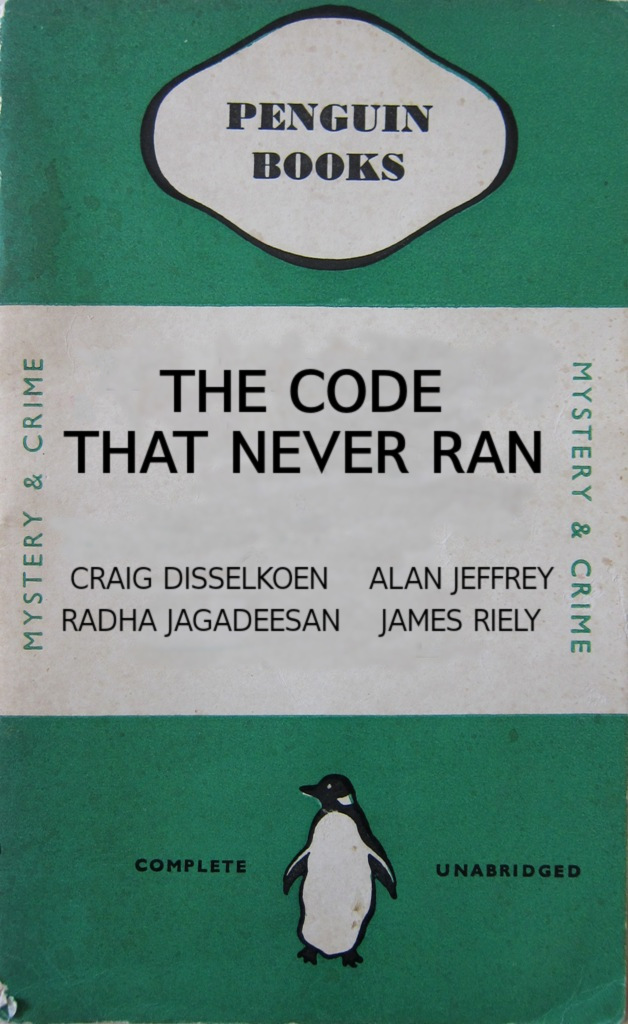
\includegraphics[height=.9\textheight]{green-penguin.jpg}
  \begin{minipage}[b][.9\textheight]{.66\textwidth}\raggedleft
    A classic locked-room mystery.\\
    Eve was in the false branch of a conditional the whole time,\\
    \emph{how could she do it}?

    \vss

    \tiny
    
\includegraphics[height=1.5ex]{cc-by-88x31.png}~Creative Commons Attribution-ShareAlike 4.0

    Mozilla Research \textbar~DePaul University \textbar~U.~California San Diego
  \end{minipage}
\end{frame}

\section{Introduction}
\begin{frame}{Overview}
  \begin{quotation}
  \tableofcontents
  \end{quotation}
\end{frame}

\begin{frame}
  \frametitle{Why? Spectre!}
  \vss
  {\fboxrule=1ex\fboxsep=0pt\fbox{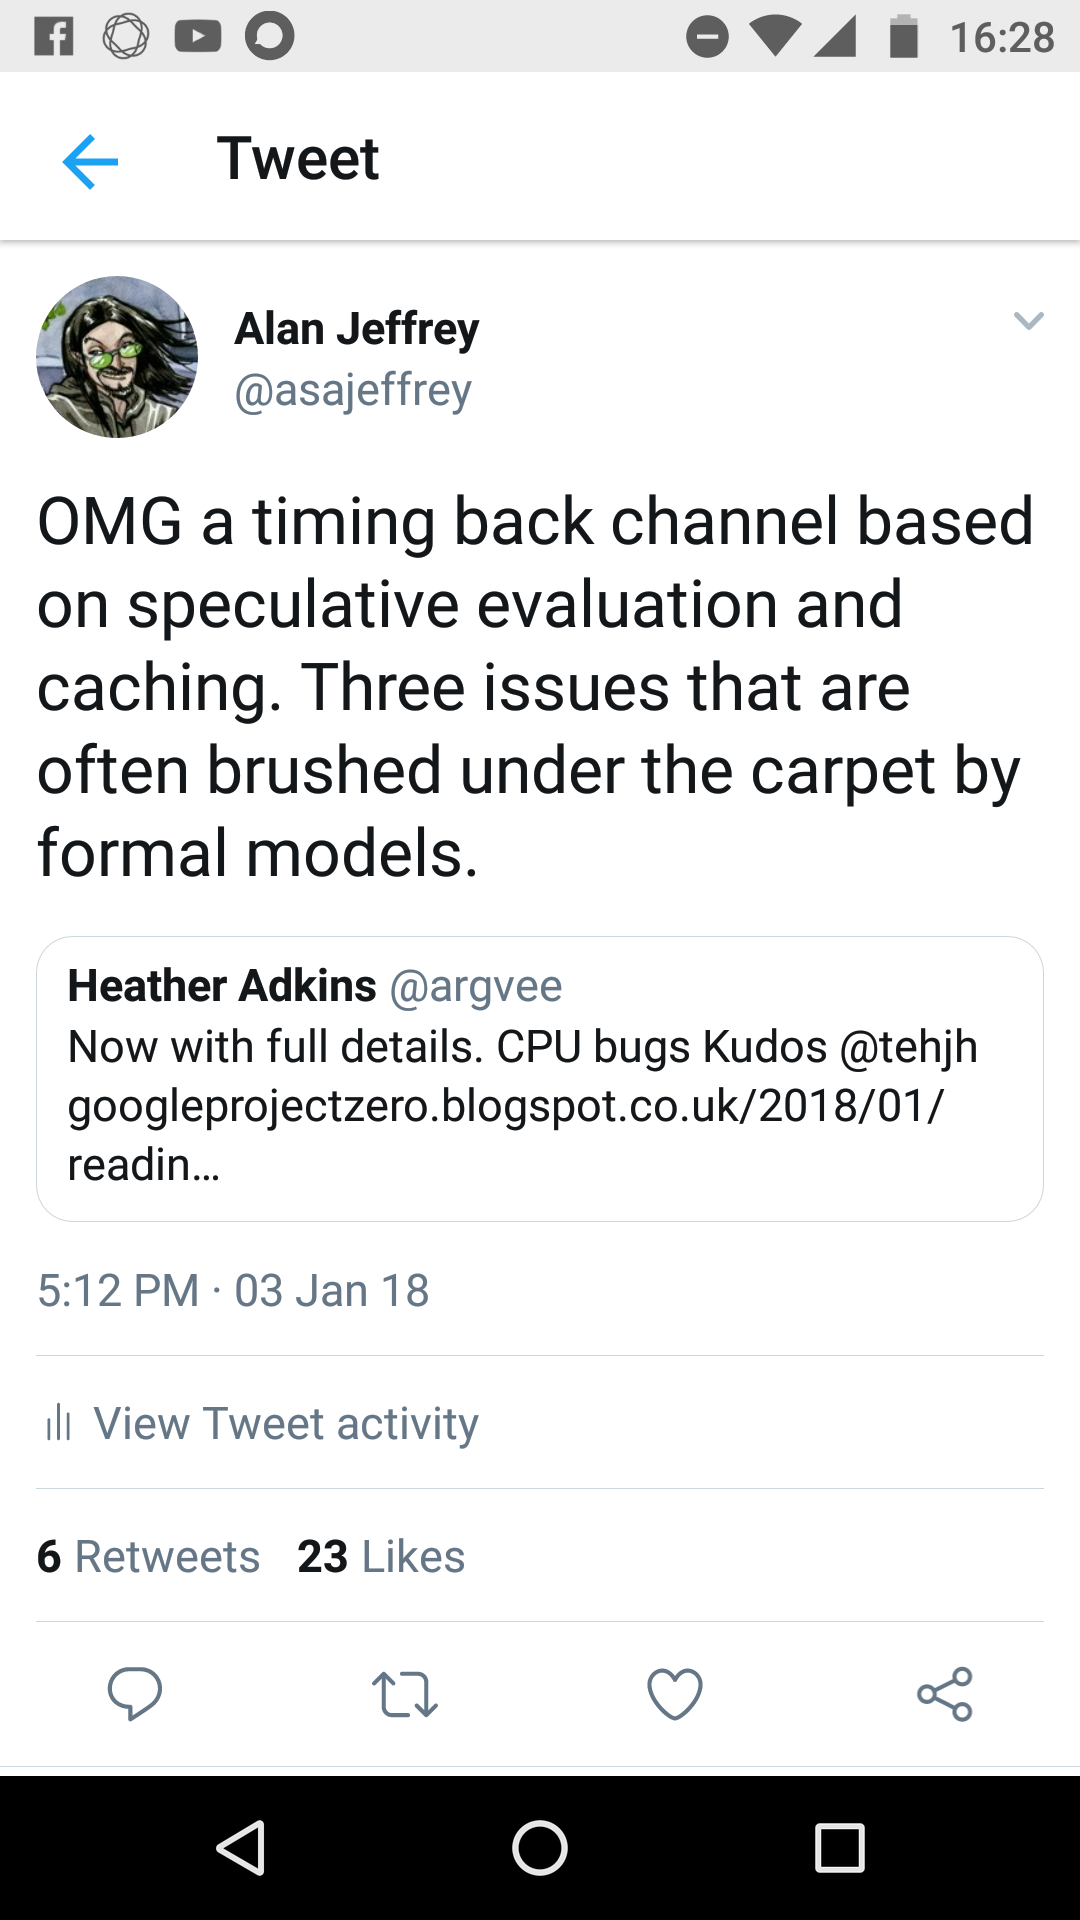
\includegraphics[height=.8\textheight]{omg-tweet.png}}}
\end{frame}

\section{Model}
\begin{frame}
  \frametitle{Model goes here}
\end{frame}

\section{Examples}
\begin{frame}
  \frametitle{Examples go here}
\end{frame}

\section{Attacks}
\begin{frame}
  \frametitle{Information flow attacks go here}
\end{frame}

\section{Experiments}
\begin{frame}
  \frametitle{Implementing the new attacks}
\end{frame}

\section{Conclusions}
\begin{frame}
  \frametitle{Outro goes here}
\end{frame}

\end{document}
